%%%%%%%%%%%%%%%%%%%%%%%%%%%%%%%%%%%%%%%%%%%%%%%%%%%%%%%%%%%%%%%%%%%%%%%%%%%%%%%%
%2345678901234567890123456789012345678901234567890123456789012345678901234567890
%        1         2         3         4         5         6         7         8

\documentclass[letterpaper, 10 pt, conference]{ieeeconf}  % Comment this line out if you need a4paper

%\documentclass[a4paper, 10pt, conference]{ieeeconf}      % Use this line for a4 paper

\IEEEoverridecommandlockouts                              % This command is only needed if 
                                                          % you want to use the \thanks command

\overrideIEEEmargins                                      % Needed to meet printer requirements.

%In case you encounter the following error:
%Error 1010 The PDF file may be corrupt (unable to open PDF file) OR
%Error 1000 An error occurred while parsing a contents stream. Unable to analyze the PDF file.
%This is a known problem with pdfLaTeX conversion filter. The file cannot be opened with acrobat reader
%Please use one of the alternatives below to circumvent this error by uncommenting one or the other
%\pdfobjcompresslevel=0
%\pdfminorversion=4

% See the \addtolength command later in the file to balance the column lengths
% on the last page of the document

% The following packages can be found on http:\\www.ctan.org
%\usepackage{graphics} % for pdf, bitmapped graphics files
%\usepackage{epsfig} % for postscript graphics files
%\usepackage{mathptmx} % assumes new font selection scheme installed
%\usepackage{times} % assumes new font selection scheme installed
%\usepackage{amsmath} % assumes amsmath package installed
%\usepackage{amssymb}  % assumes amsmath package installed

% basic
\usepackage{color,xcolor}
\usepackage{epsfig}
\usepackage{graphicx}

% figure and table
\usepackage{adjustbox}
\usepackage{array}
\usepackage{booktabs}
\usepackage{colortbl}
\usepackage{wrapfig}
\usepackage{hhline}
\usepackage{multirow}
\usepackage{subcaption} % issues a warning with CVPR/ICCV format
\usepackage[skip=1pt,labelfont=bf,font=footnotesize]{caption}
\usepackage{wrapfig}
\usepackage{floatflt}

% font and character
% \usepackage{txfonts}
\let\proof\relax
\let\endproof\relax
\usepackage{amsmath,amsfonts,amssymb,amsthm}
\usepackage{mathtools}  % additional useful math commands, such as \coloneqq
\usepackage{bm}
% \usepackage{bbold}  % special blackboard bold characters (e.g., 1)
\usepackage{nicefrac}
\usepackage{microtype}
\usepackage{times} % assumes new font selection scheme installed
\usepackage{mathptmx} % assumes new font selection scheme installed

% layout
\usepackage{changepage}
\usepackage{extramarks}
\usepackage{fancyhdr}
\usepackage{lastpage}
\usepackage{setspace}
\usepackage{soul}
\usepackage{xspace}
\usepackage{adjustbox}

% ref
\usepackage[breaklinks=true,colorlinks,citecolor=gray]{hyperref}
\newcommand\nnfootnote[1]{%
  \begin{NoHyper}
  \renewcommand\thefootnote{}\footnote{#1}%
  \addtocounter{footnote}{-1}%
  \end{NoHyper}
}
\usepackage{url}
\definecolor{urlblue}{rgb}{0,0,0.5}
\hypersetup{urlcolor=urlblue}
\usepackage[noadjust]{cite}

% misc
%\usepackage{algorithm, algorithmic}
\usepackage{enumerate}
\usepackage{todonotes} % conflict with CVPR/ICCV format
\let\labelindent\relax
\usepackage{enumitem}  % control indent of enumerate, itemize, etc.

\usepackage{titlesec}

%\usepackage{fourier} 
\usepackage{makecell}

\usepackage{pifont} % for extra symbols such as \cmark
% \usepackage{subcaption}

\usepackage[ruled,vlined]{algorithm2e}
\DontPrintSemicolon
\urlstyle{same}

% shaded
\usepackage{framed}
\definecolor{shadecolor}{gray}{0.95}

\usepackage{xparse}
\usepackage{etoolbox}

% for \texttt
\usepackage{courier}

\input{inc-math}
% require xspace, array

\newcommand{\stderr}[1]{\scriptsize $\pm #1$}

%% layout
\newcolumntype{L}[1]{>{\raggedright\let\newline\\\arraybackslash\hspace{0pt}}m{#1}}
\newcolumntype{C}[1]{>{\centering\let\newline\\\arraybackslash\hspace{0pt}}m{#1}}
\newcolumntype{R}[1]{>{\raggedleft\let\newline\\\arraybackslash\hspace{0pt}}m{#1}}

\newcommand{\xpar}[1]{\noindent\textbf{#1}\ \ }
\newcommand{\vpar}[1]{\vspace{3mm}\noindent\textbf{#1}\ \ }

%% notations
\newcommand{\sect}[1]{Section~\ref{#1}}
\newcommand{\sectapp}[1]{Appendix~\ref{#1}}
\newcommand{\ssect}[1]{\S~\ref{#1}}
\newcommand{\eqn}[1]{Equation~\ref{#1}}
\newcommand{\fig}[1]{Fig.~\ref{#1}}
\newcommand{\tbl}[1]{Table~\ref{#1}}
\newcommand{\alg}[1]{Algorithm.~\ref{#1}}

\newcommand{\degree}{\ensuremath{^\circ}\xspace}
\newcommand{\ignore}[1]{}
\newcommand{\norm}[1]{\lVert#1\rVert}
\newcommand{\fcseven}{$\mbox{fc}_7$}

% \DeclarePairedDelimiter\ceil{\lceil}{\rceil}
% \DeclarePairedDelimiter\floor{\lfloor}{\rfloor}
% \DeclareMathOperator*{\argmin}{arg\,min}
% \DeclareMathOperator*{\argmax}{arg\,max}

\renewcommand*{\thefootnote}{\fnsymbol{footnote}}

\def\naive{na\"{\i}ve\xspace}
\def\Naive{Na\"{\i}ve\xspace}

\makeatletter
\DeclareRobustCommand\onedot{\futurelet\@let@token\@onedot}
\def\@onedot{\ifx\@let@token.\else.\null\fi\xspace}

\def\eg{e.g\onedot} \def\Eg{E.g\onedot}
\def\ie{i.e\onedot} \def\Ie{I.e\onedot}
\def\cf{\emph{c.f}\onedot} \def\Cf{\emph{C.f}\onedot}
\def\etc{etc\onedot}
\def\vs{\emph{vs}\onedot}
\def\wrt{w.r.t\onedot}
\def\dof{d.o.f\onedot}
\def\etal{et al\onedot}
\def\aka{a.k.a\onedot}
\makeatother

%% comments
\definecolor{MyDarkBlue}{rgb}{0,0.08,1}
\definecolor{MyDarkGreen}{rgb}{0.02,0.6,0.02}
\definecolor{MyDarkRed}{rgb}{0.8,0.02,0.02}
\definecolor{MyDarkOrange}{rgb}{0.40,0.2,0.02}
\definecolor{MyPurple}{RGB}{111,0,255}
\definecolor{MyRed}{rgb}{1.0,0.0,0.0}
\definecolor{MyGold}{rgb}{0.75,0.6,0.12}
\definecolor{MyDarkgray}{rgb}{0.66, 0.66, 0.66}
\definecolor{JiayuanColor}{rgb}{0.60,0.43,0.48}

\newcommand{\red}[1]{\textcolor{red}{#1}}
\newcommand{\showcomment}[3]{\colorbox{#1}{\textcolor{white}{#2}}~{\textcolor{#1}{#3}}}
\newcommand{\jiayuan}[1]{\showcomment{JiayuanColor}{Author}{#1}}

\newcommand{\cn}{\textcolor{MyRed}{[Citation!]}\xspace}
\newcommand{\fn}{\textcolor{MyRed}{[Figure!]}\xspace}
\newcommand{\tbd}[1]{\textcolor{MyRed}{#1}\xspace}

\newcommand{\newtext}[1]{\textcolor{MyDarkBlue}{#1}}

% Begin:: Jiayuan - STRIPS style notations
\newcommand{\object}[1]{\text{#1}}

\NewDocumentCommand{\prop}{m >{\SplitList{,}}m}{%
  \ensuremath{\textit{#1}(%
  \ProcessList{#2}{\propositionitem}%
  )}%
  \propositionfirstitemtrue
}

\newif\ifpropositionfirstitem
\propositionfirstitemtrue  
\newcommand\propositionitem[1]{%
  \ifpropositionfirstitem
    \propositionfirstitemfalse
  \else
    , %
  \fi
  \text{#1}}

\newcommand{\gregress}[3]{\ensuremath{#1 \leftsquigarrow #2~\|~#3}}
\newcommand{\gregressfull}[4]{\ensuremath{#1^#2 \leftsquigarrow #3~\|~#4}}
\newcommand{\pre}{\ensuremath{\textit{pre}}}
\newcommand{\effp}{\ensuremath{\textit{eff}_+}}
\newcommand{\effm}{\ensuremath{\textit{eff}_-}}
\newcommand{\var}[1]{\ensuremath{\textit{#1}}}
\newcommand{\func}[1]{\ensuremath{\textit{#1}}}
\newcommand{\md}[2]{#1$\pm$#2}
\newcommand{\bmd}[2]{\textbf{#1$\pm$#2}}


% End:: Jiayuan - STRIPS style notations

\def\bR{\mathbb{R}}
\def\cL{\mathcal{L}}

\newcommand{\mysubsection}[1]{\vspace{-4pt}\subsection{#1}\vspace{-4pt}}
% \newcommand{\myparagraph}[1]{\vspace{-5pt}\paragraph{#1}}
\newcommand{\myparagraph}[1]{\noindent\textbf{#1}}
\newcommand{\xhdr}[1]{\noindent\textbf{#1}}
\newcommand{\myitem}{\vspace{-5pt}\item}
\newcommand{\mybf}[1]{\vspace{4pt}\noindent\textbf{#1}}
\newcommand{\mycell}[1]{\begin{tabular}[t]{@{}l@{}l}#1\end{tabular}}
\newcommand{\mycellc}[1]{\begin{tabular}[t]{@{}c@{}l}#1\end{tabular}}

\theoremstyle{plain}% default
\newtheorem{definition}{Definition}[section]
\newtheorem{theorem}{Theorem}[section]
\newtheorem{lemma}{Lemma}[section]

%\usepackage{titlesec}
%\titlespacing*{\section}{0pt}{0pt plus 2pt minus 2pt}{0pt plus 2pt minus 2pt}
%\titlespacing*{\subsection}{0pt}{0pt plus 1pt minus 1pt}{0pt plus 1pt minus 1pt}


\title{\LARGE \bf
\ours: Robot Agentic Programming from Demonstrations 
% \\ with Application to Nonprehensile Manipulation
% Closing the Agentic Coding Loop for Robotic Manipulation
}


% \author{Anonymous Authors}


\begin{document}
\nocite{IEEEcontrol}

\maketitle
\thispagestyle{empty}
\pagestyle{empty}

\begin{abstract}

Coding agents have demonstrated enormous success in solving complex programming problems. To leverage their potential for robot systems, this work introduces \textbf{Robot Agentic Programming from Demonstrations (\ours)}, which automatically generates, verifies, and refines robot programs, given a \textrm{single visual human demonstration}. The iterative agentic loop of code refinement requires several key ingredients: (i) a testable task specification, (ii) action primitives for robot execution, and (iii) an interactive environment for program execution and verification. \ours infers all three from the demonstration automatically. To make the resulting program reusable beyond the demonstration setting, \ours uses an \textit{object-centric relational program representation} that focuses on the underlying structure of the demonstrated strategy rather than the specific motion \textit{per se}: it expresses the action primitives as trajectory-optimization programs that realize object-level motion effects, while composing them through relational constraints that capture scene-specific geometry at run time.  We evaluated \ours in simulation on eight challenging contact-rich nonprehensile manipulation tasks as well as general prehensile manipulation tasks in the LIBERO-Pro benchmark. We also successfully deployed it on a real Franka arm and evaluated on all eight nonprehensile tasks. In all experiments, \ours demonstrated strong performance, with generalization over object pose, shape, material, and environment. 
\end{abstract}

\section{Introduction}

Recently, coding agents~\cite{openai_codex,anthropic_claude_code} have shown remarkable capabilities in developing complex software systems, sparking growing interest in solving robotic manipulation tasks through programming~\cite{chen2026gap,xiao2026enpire,lu2026aspire,fu2026cap,berman2026claude,noematrix2026roborsi,liang2023code}. Consider how human engineers would develop a robot program to solve the task in Figure~\ref{fig:teaser} before the era of coding agents: given the \textit{(a) task specification} (pick up the cookie box), they would write a program that composes the available \textit{(b) manipulation primitives} (push the box to a fixture, flip it against the fixture, then grasp and lift it), and test the program in \textit{(c) interactive environments} to verify its correctness and iteratively debug it. This process mirrors the core strength of coding agents: not one-shot code generation, but the iterative cycle of generating, executing, verifying, and revising a program, commonly referred to as the agentic coding loop~\cite{ng2026three,huang2023agentcoder}.

For the agentic coding loop to work in robotic manipulation, it requires three ingredients: task specification, manipulation primitives, and interactive environments for verification. Existing robotic coding-agent systems typically assume these ingredients are provided through human-engineered primitives, explicit task objectives, and resettable environments with reward or success feedback. This raises a fundamental question: \textbf{how can a coding agent close the loop when these ingredients are not provided a priori?}

We explore \textit{demonstrations} as a programming interface for supplying the task- and motion-level information needed by the agentic coding loop. A demonstration directly shows a feasible way to accomplish a task and, together with a language description, conveys the intended outcome. Rather than merely reproducing the demonstrated trajectory, we aim to recover an executable and reusable manipulation program. Demonstrations, however, do not provide the interactive environment needed to verify and iteratively refine that program, posing an additional challenge for verification.

\begin{figure}[t]    
    \centering
    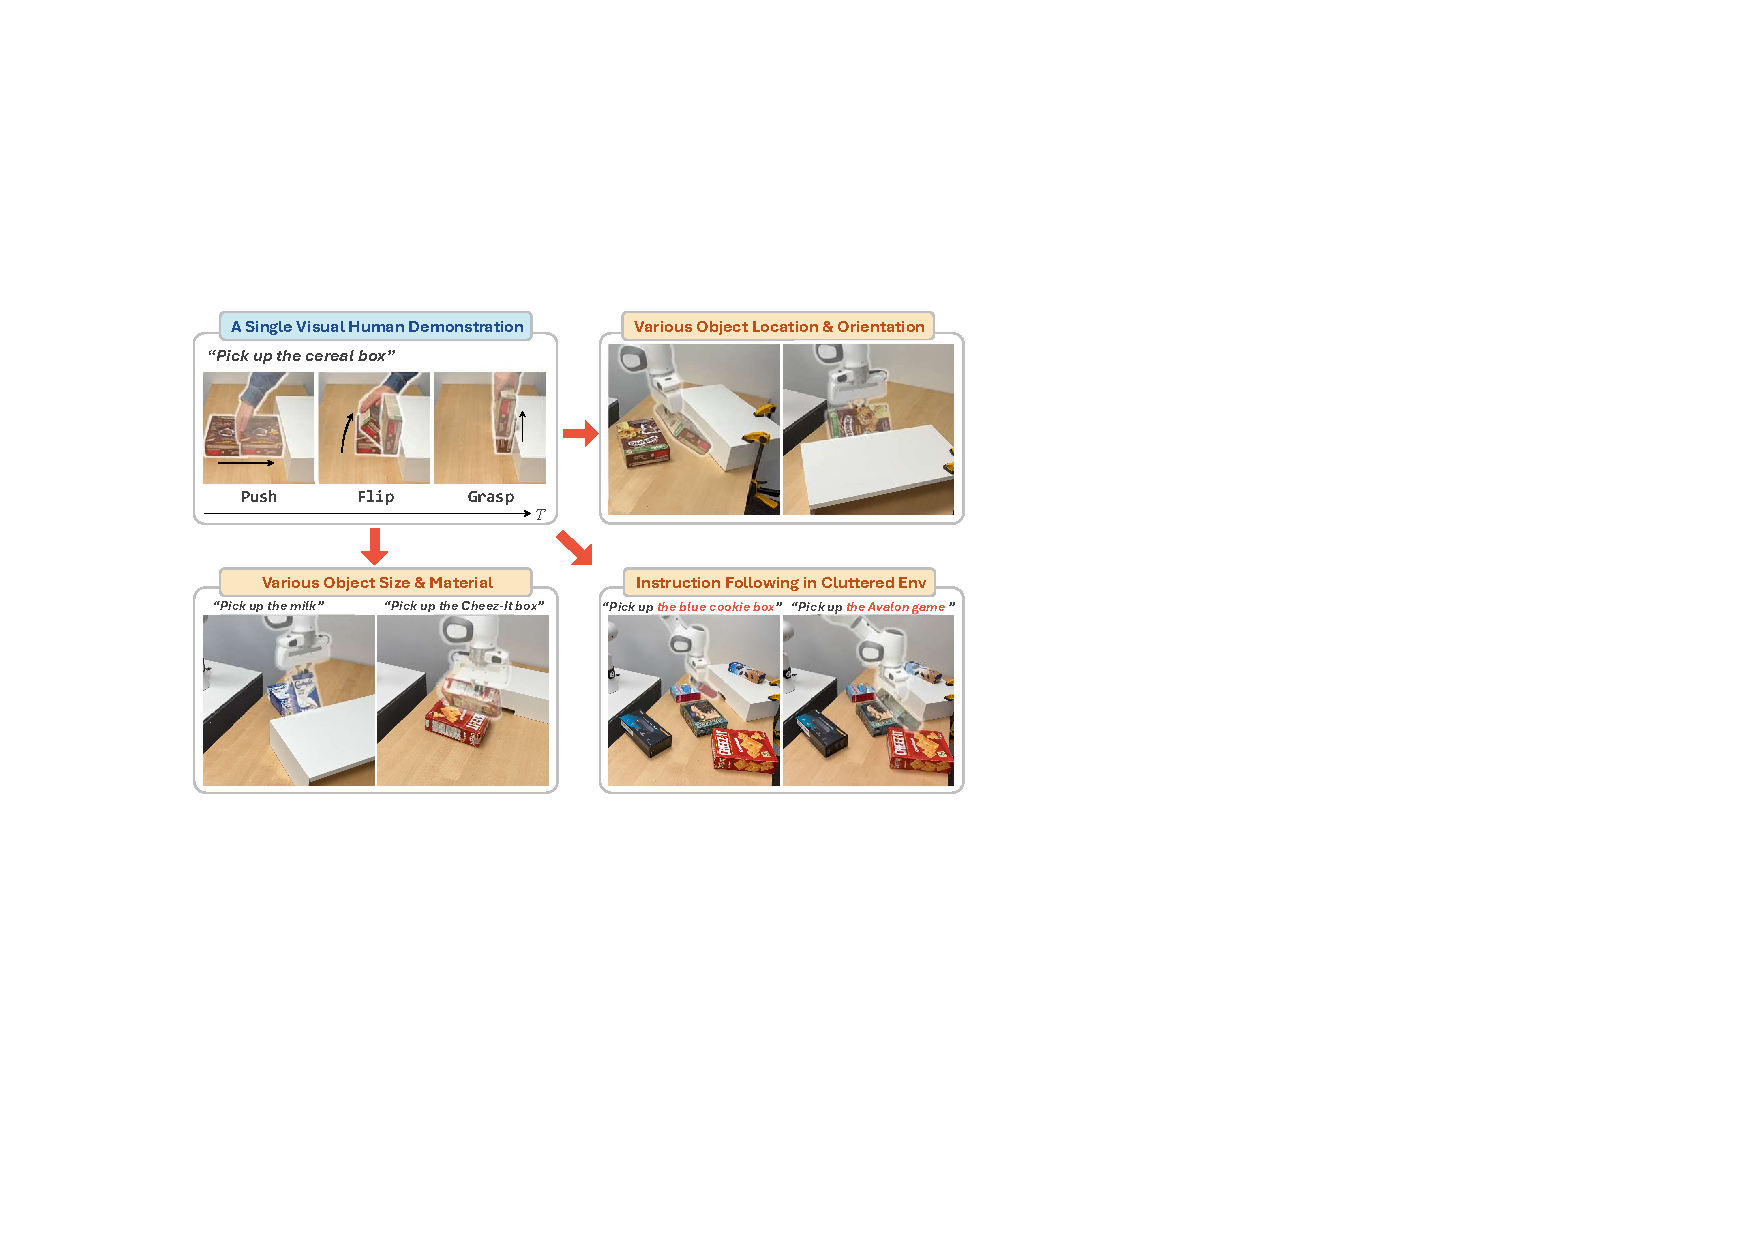
\includegraphics[width=\linewidth]{figures/teaser.pdf}
    \caption{teaser}
    \vspace{-0.3in}
    \label{fig:teaser}
\end{figure}

Motivated by this perspective, we introduce \textbf{R}obot \textbf{A}gentic \textbf{P}rogramm\textbf{i}ng from \textbf{D}emonstrations (\textbf{RAPID}), a framework for constructing and iteratively refining robot programs from a single human demonstration with a coding agent. RAPID infers the task specification, constructs the required manipulation primitives and strategy, and reconstructs the demonstrated scene in simulation for iterative program verification and refinement. To improve generalization, RAPID additionally generates scene variants for further verification. In this way, RAPID automatically establishes the three ingredients required to close the agentic coding loop for robotic manipulation.

In this work, we apply RAPID to \textit{nonprehensile manipulation}, where the need for such a framework is especially acute. Many prehensile tasks can be composed from a compact and well-established set of reusable primitives~\cite{garrett2021integrated}, including \textit{pick}, \textit{move in free space}, and \textit{place}. Nonprehensile manipulation, by contrast, spans diverse and geometry-dependent contact interactions, including pushing~\cite{mason2001mechanics}, pivoting~\cite{holladay2015general}, toppling~\cite{cheng2021contact}, flipping~\cite{odhner2013open}, and sliding~\cite{cheng2022contact}. Capturing this diversity with a fixed primitive library is difficult, making manual primitive design a significant engineering burden. This makes nonprehensile manipulation a natural testbed for asking whether a coding agent can construct reusable manipulation primitives from a single demonstration rather than rely on human engineering.

A central challenge is \textit{generalization} beyond a single demonstrated scene. Programs that directly encode poses, distances, or waypoints may reproduce the demonstrated behavior but can fail when the scene changes. RAPID instead captures the behavior in terms of object-centric relations and task-relevant effects. Specifically, RAPID represents primitives as relational trajectory-optimization programs that realize object-level motion effects, such as pushing an object by a displacement or flipping it by an angle, while resolving scene-dependent geometry at execution time. At the task level, primitives are connected into a strategy through relational constraints that determine how the outcome of one phase specifies the next. For example, rather than replaying a fixed pushing distance, the program can compute how far an object should be pushed from its current pose to establish contact with a fixture. By expressing primitives and their composition relationally, RAPID preserves the invariant structure of the demonstrated strategy while adapting to changes in object pose, size, geometry, and physical properties.

The remaining challenge is \textit{verification}: the coding agent needs an interactive environment in which candidate programs can be executed, evaluated, and revised. RAPID reconstructs such an environment in simulation from the demonstration and augments it with scene variants that perturb object geometry, pose, appearance, and physical properties. Agent-generated filters retain only task-consistent and physically feasible variants. The coding agent then executes and iteratively revises the program across this verification set. This simulation-based verification closes the agentic loop while reducing overfitting to the demonstrated scene.

We evaluate RAPID on 8 contact-rich nonprehensile manipulation tasks, focusing on whether a program constructed from one demonstrated instance can generalize to substantial changes in object pose, geometry, physical properties, and scene configuration. We additionally evaluate the frozen programs on physical robots and conduct ablations to assess the contributions of the relational program representation, scene variation, and iterative verification.

Our contributions are threefold:

\begin{itemize}

\item We introduce RAPID, a framework that closes the agentic coding loop for robotic manipulation by automatically constructing \textit{(a) task specifications}, \textit{(b) manipulation primitives}, and \textit{(c) interactive verification environments}, all from a single human demonstration.

\item We introduce \textit{relational manipulation programs}, which represent manipulation primitives as parameterized trajectory-optimization programs and compose them through relational constraints, enabling reusable strategies that adapt across scenes.

\item We demonstrate that RAPID can construct reusable programs from a single human demonstration across diverse contact-rich nonprehensile manipulation tasks, generalize to substantial scene variations, and be deployed in the real world.

\end{itemize}

\section{Related Work}

\xhdr{Programming for Robotics.}
Programs provide an interface between high-level task reasoning and robot execution. Code as Policies~\cite{liang2023code} and related methods~\cite{singh2023progprompt,wang2025chainofmodality} translate language and multimodal inputs into robot programs. Other approaches generate geometric objectives and constraints~\cite{huang2023voxposer,huang2024rekep}, rewards~\cite{ma2024eureka,xie2024text2reward}, and simulation environments~\cite{wang2024robogen}. Agentic programming extends this approach by executing candidate programs and iteratively revising them from feedback. CaP-X~\cite{fu2026cap}, ENPIRE~\cite{xiao2026enpire}, and RoboRSI~\cite{noematrix2026roborsi} apply this loop to robot policy improvement, while GaP~\cite{chen2026gap} incorporates simulation rehearsal. Voyager~\cite{wang2023voyager} and ASPIRE~\cite{lu2026aspire} accumulate reusable skills through iterative program generation, as does Playful Agentic Robot Learning~\cite{zhang2026playful}. However, these agentic approaches typically assume that task success signals, human-engineered manipulation primitives, or interactive verification environments are provided a priori. In contrast, \ours closes the agentic coding loop by deriving these ingredients from a single visual human demonstration.

\xhdr{Learning from Few Demonstrations.}
Learning from few demonstrations benefits from representations that preserve task-relevant structure across objects and scenes. Spatial abstractions support transfer through visual alignment~\cite{johns2021coarsetofine}, object geometry and correspondence~\cite{wen2022you,simeonov2022neural,shen2023distilled,zhu2024densematcher}, and contact or interaction structure~\cite{biza2023one,liu2025oneshot,sieb20graph,zhu2024orion}. Demonstrations can also be decomposed into subgoals and primitives~\cite{zhang2024universal,gao2024prime}. Structured skill representations enable long-horizon planning and composition through contact retargeting, symbolic models, or geometric reasoning~\cite{wu2024oneshot,liu2024learning,cheng2024nodtamp,nie2026learning}. However, these representations are generally embedded in fixed learning or planning pipelines. In contrast, \ours combines a relational program representation of manipulation effects and composition constraints with agentic programming to iteratively construct, verify, and refine transferable manipulation strategies.

\xhdr{Nonprehensile Manipulation.}
Nonprehensile manipulation exploits environmental contact to reposition objects and enable otherwise difficult grasps~\cite{chavandafle2014extrinsic}. Prior work develops mechanics-based models~\cite{lynch1996stable,holladay2015general}, contact-aware planners~\cite{lee2015hierarchical,cheng2021contact,cheng2022contact}, and optimization methods for trajectories and primitives~\cite{sleiman2019contact,aceituno2020global,pang2023global,huang2023autogenerated}. Learning-based approaches acquire contact-rich policies~\cite{zhou2023learning,zhou2023hacman,cho2024corn} or compose predefined primitives~\cite{nasiriany2022augmenting}. However, these methods typically rely on explicit task specifications or task-specific policy training. In contrast, \ours approaches nonprehensile manipulation through agentic programming from a single visual human demonstration, automatically constructing and iteratively refining the required primitives and their composition.

\section{Overview}
\label{sec:overview}
\label{sec:problem}

\xhdr{Problem statement.}
We consider programming a reusable strategy for quasi-static manipulation of rigid bodies from \textit{a single visual human demonstration} $D$ and a language description $l$. The program should solve a family of tasks $\mathcal{E}$ that share similar objectives but may vary in object appearance, geometry, pose, physical properties, and scene configuration. No manipulation primitives, explicit success or reward signals, or instantiated simulation environments are provided \textit{a priori}. Given only $(D,l)$, the agent aims to construct executable primitives $\mathcal{P}=\{P_1,\ldots,P_N\}$ and compose them into a strategy $\Pi$ that captures the underlying structure of the demonstration and generalizes to unseen language instructions $l^\star$ and test scenes $E^\star$ in $\mathcal{E}$:
\[
(D,l)
\mapsto
(\mathcal{P},\Pi),
\quad
\Pi(E^\star, l^\star;\mathcal{P}) \text{ succeeds for } (E^\star, l^\star) \in \mathcal{E}.
\]

\xhdr{Overview of \ours.}
As shown in \fig{fig:method_overview}, RAPID closes the agentic coding loop by deriving task specifications, manipulation primitives, and verification environments from $(D,l)$. It partitions the demonstration into interaction phases, infers a subgoal and success predicate for each phase, and reconstructs the corresponding interactive simulation environments. To improve generalization, RAPID also synthesizes feasible scene variants for additional verification. For each phase, the coding agent generates a primitive to achieve its subgoal and iteratively executes, verifies, and revises it in the corresponding environment and its variants. It then infers the overall task goal and success predicate, composes the verified primitives into a strategy, and refines the composition through the same loop. At deployment, given an RGB-D observation of a novel scene and a language instruction, RAPID reconstructs the scene in simulation, instantiates and runs the strategy program in this scene, and executes the output trajectory on the robot. We describe program construction and verification in Sec.~\ref{sec:agentic_programming}.

We introduce a \textit{relational program representation} to make manipulation strategies reusable across scenes. A strategy connects primitives through relational constraints that specify what each primitive should accomplish in the current scene. Each primitive then uses local trajectory optimization to achieve the requested object-level effect, taking the scene's geometry and physical properties into account. To deploy the program in a new scene, we use lightweight semantic binding to match scene objects to program roles. The strategy and primitives themselves remain unchanged. We provide the details of the representation in Sec.~\ref{sec:relational_programs}.

\section{Relational Manipulation Programs}
\label{sec:relational_programs}

We now define relational primitives, their composition into task-level strategies, and their instantiation in novel scenes.

\subsection{Primitives as Local Trajectory-Optimization Programs}
\label{sec:relational_primitives}
A primitive is a reusable behavior for realizing an object-level motion effect, such as pushing for a displacement or flipping for an angle. We represent a primitive as a local relational trajectory-optimization program
\begin{equation*}
    P_i=(G_i,C_i,\Psi_i,\rho_i,J_i)\in\mathcal{P}.
\end{equation*}
Here, $G_i$ is a semantic, object-centric description of the intended effect; $C_i$ is the relational interface; $\Psi_i$ is the verifiable success condition; $\rho_i$ is the geometry resolver; and $J_i$ is the optimization cost. Together, these components specify how the primitive is instantiated, optimized, and verified in a specific scene. A primitive is therefore neither a fixed trajectory nor a black-box policy. Table~\ref{tab:flip_primitive} illustrates each component for flipping an object against a fixture.

\begin{table}[t]
    \caption{\textbf{Object-centric trajectory optimization program for flipping.}}
    \label{tab:flip_primitive}
    \begin{adjustbox}{width=\columnwidth}
    \centering
    \setlength{\tabcolsep}{2pt}
    \begin{tabular}{@{}>{\raggedright\arraybackslash}p{0.37\columnwidth}
                        >{\raggedright\arraybackslash}p{1.13\columnwidth}@{}}
        \toprule
        \textbf{Component} & \textbf{Content} \\
        \midrule
        Semantic goal $G_i$
            & Flip the target against the vertical fixture for a specific angle. \\
        \rowcolor{black!5}
        Relational contract $C_i$
            & Semantic roles $\mathbf{r}_i$: target, support plane, fixture, and pusher.
              Relations $\Gamma_i$: the target rests on the support plane, and the fixture
              exposes a reachable vertical face. Effect parameter $\mathbf{q}_i$: flipping angle.\\
        Success predicate $\Psi_i$
            & Check that the achieved rotation matches the flipping angle and that the
              target remains supported, near the fixture, and settled. \\
        \rowcolor{black!5}
        Geometry resolver $\rho_i$
            & At each rollout state, derive the support plane, fixture face,
              pivot axis, target faces, dimensions, and clearances. \\
        Final cost $J_i^{\mathrm{f}}$
            & Penalize terminal rotation error relative to the flipping angle, support
              and fixture gaps, and terminal velocity. \\
        \rowcolor{black!5}
        Progress cost $J_i^{\mathrm{p}}$
            & Encourage rotation and pusher proximity while discouraging
              backtracking and irregular motion. \\
        \bottomrule
    \end{tabular}
    \end{adjustbox}
    \vspace{-0.3in}
\end{table}

\xhdr{Relational interface.}
We write the primitive interface as
\begin{equation*}
    C_i=(\mathbf{r}_i,\Gamma_i,\mathbf{q}_i).
\end{equation*}
The declarations $\mathbf{r}_i$ and $\mathbf{q}_i$ specify the semantic scene roles and typed effect-parameter slots required by $P_i$, while $\Gamma_i$ specifies the relations among the roles. An invocation supplies runtime arguments $(b_i,g_i)$ satisfying
\begin{equation*}
    b_i\in\operatorname{Bind}_E(\mathbf{r}_i,\Gamma_i),
    \qquad
    g_i\in\operatorname{Val}(\mathbf{q}_i).
\end{equation*}
Here, $\operatorname{Bind}_E(\mathbf{r}_i,\Gamma_i)$ denotes the type-compatible assignments of scene entities from the environment $E$ to $\mathbf{r}_i$ that satisfy $\Gamma_i$, and $\operatorname{Val}(\mathbf{q}_i)$ denotes the values matching the types declared by $\mathbf{q}_i$. In the flipping example (Table~\ref{tab:flip_primitive}), $b_i$ binds the target, support plane, fixture, and pusher to scene entities, while $g_i$ supplies the requested angle. Scene-dependent geometry remains internal to the primitive and is resolved by $\rho_i$ at execution time.

\xhdr{Geometry resolver.}
Let $\mathcal{X}(E)$ be the state space of environment $E$. At each state $x_t\in\mathcal{X}(E)$ along a rollout, the geometry resolver computes
\begin{equation*}
    \phi_{i,t} = \rho_i(E,x_t,b_i), \qquad t=0,\ldots,T,
\end{equation*}
where $\phi_{i,t}$ collects the geometric features at time $t$.

\xhdr{Success predicate.}
For a terminal state $x_T\in\mathcal{X}(E)$, the predicate $\Psi_i(E,x_T;g_i,\phi_{i,T})\in\{0,1\}$ provides an executable interpretation of $G_i$. It evaluates the achieved object relations and requested effect, yielding an unambiguous signal for verification. 

\xhdr{Optimization cost.}
For a simulated trajectory $\tau=(x_0,\ldots,x_T)$ in environment $E$, where $x_t\in\mathcal{X}(E)$, the primitive cost is
\begin{equation*}
    \begin{aligned}
        J_i(E,\tau;g_i,\phi_{i,0:T})
        = J_i^{\mathrm{f}}(E,x_T;g_i,\phi_{i,T}) 
        + \lambda_i J_i^{\mathrm{p}}(E,\tau;g_i,\phi_{i,0:T}).
    \end{aligned}
\end{equation*}
Here, $J_i^{\mathrm{f}}$ is the final cost, which measures how far $x_T$ is from the effect encoded by $G_i$; $J_i^{\mathrm{p}}$ is the progress cost, which may depend on the full trajectory and guides the optimizer through contact-rich interaction heuristics; and $\lambda_i\geq 0$ is a constant. The coding agent proposes the heuristics by reasoning about the visual human demonstration.

During primitive construction, the agent also proposes an initialization heuristic based on the resolved geometry and requested effect. The heuristic provides a plausible interaction trajectory from which to begin the search. Let $z$ parameterize a candidate robot motion, let $\tau(z)=\operatorname{Rollout}_E(x_0,z)$ denote its simulated state trajectory from $x_0$ in environment $E$, and let $\phi_{i,0:T}(z)$ be the feature sequence resolved along that trajectory. The executable trajectory is obtained as
\begin{equation*}
    z_i^\star
    = \arg\min_z
    J_i\!\left(E,\tau(z);g_i,\phi_{i,0:T}(z)\right).
\end{equation*}
We solve this trajectory-optimization problem with the Cross-Entropy Method (CEM)~\cite{deboer2005tutorial}, a sampling-based optimizer. We use CEM because it is gradient-free, allowing us to optimize robot motions without differentiating through the contact-rich simulation. The primitive thereby adapts its motion to the object pose, size, geometry, physical properties, and requested effect.

\subsection{Strategies as Primitive Composition by Constraints}
\label{sec:relational_strategy}

\begin{figure}[t]
    \centering
    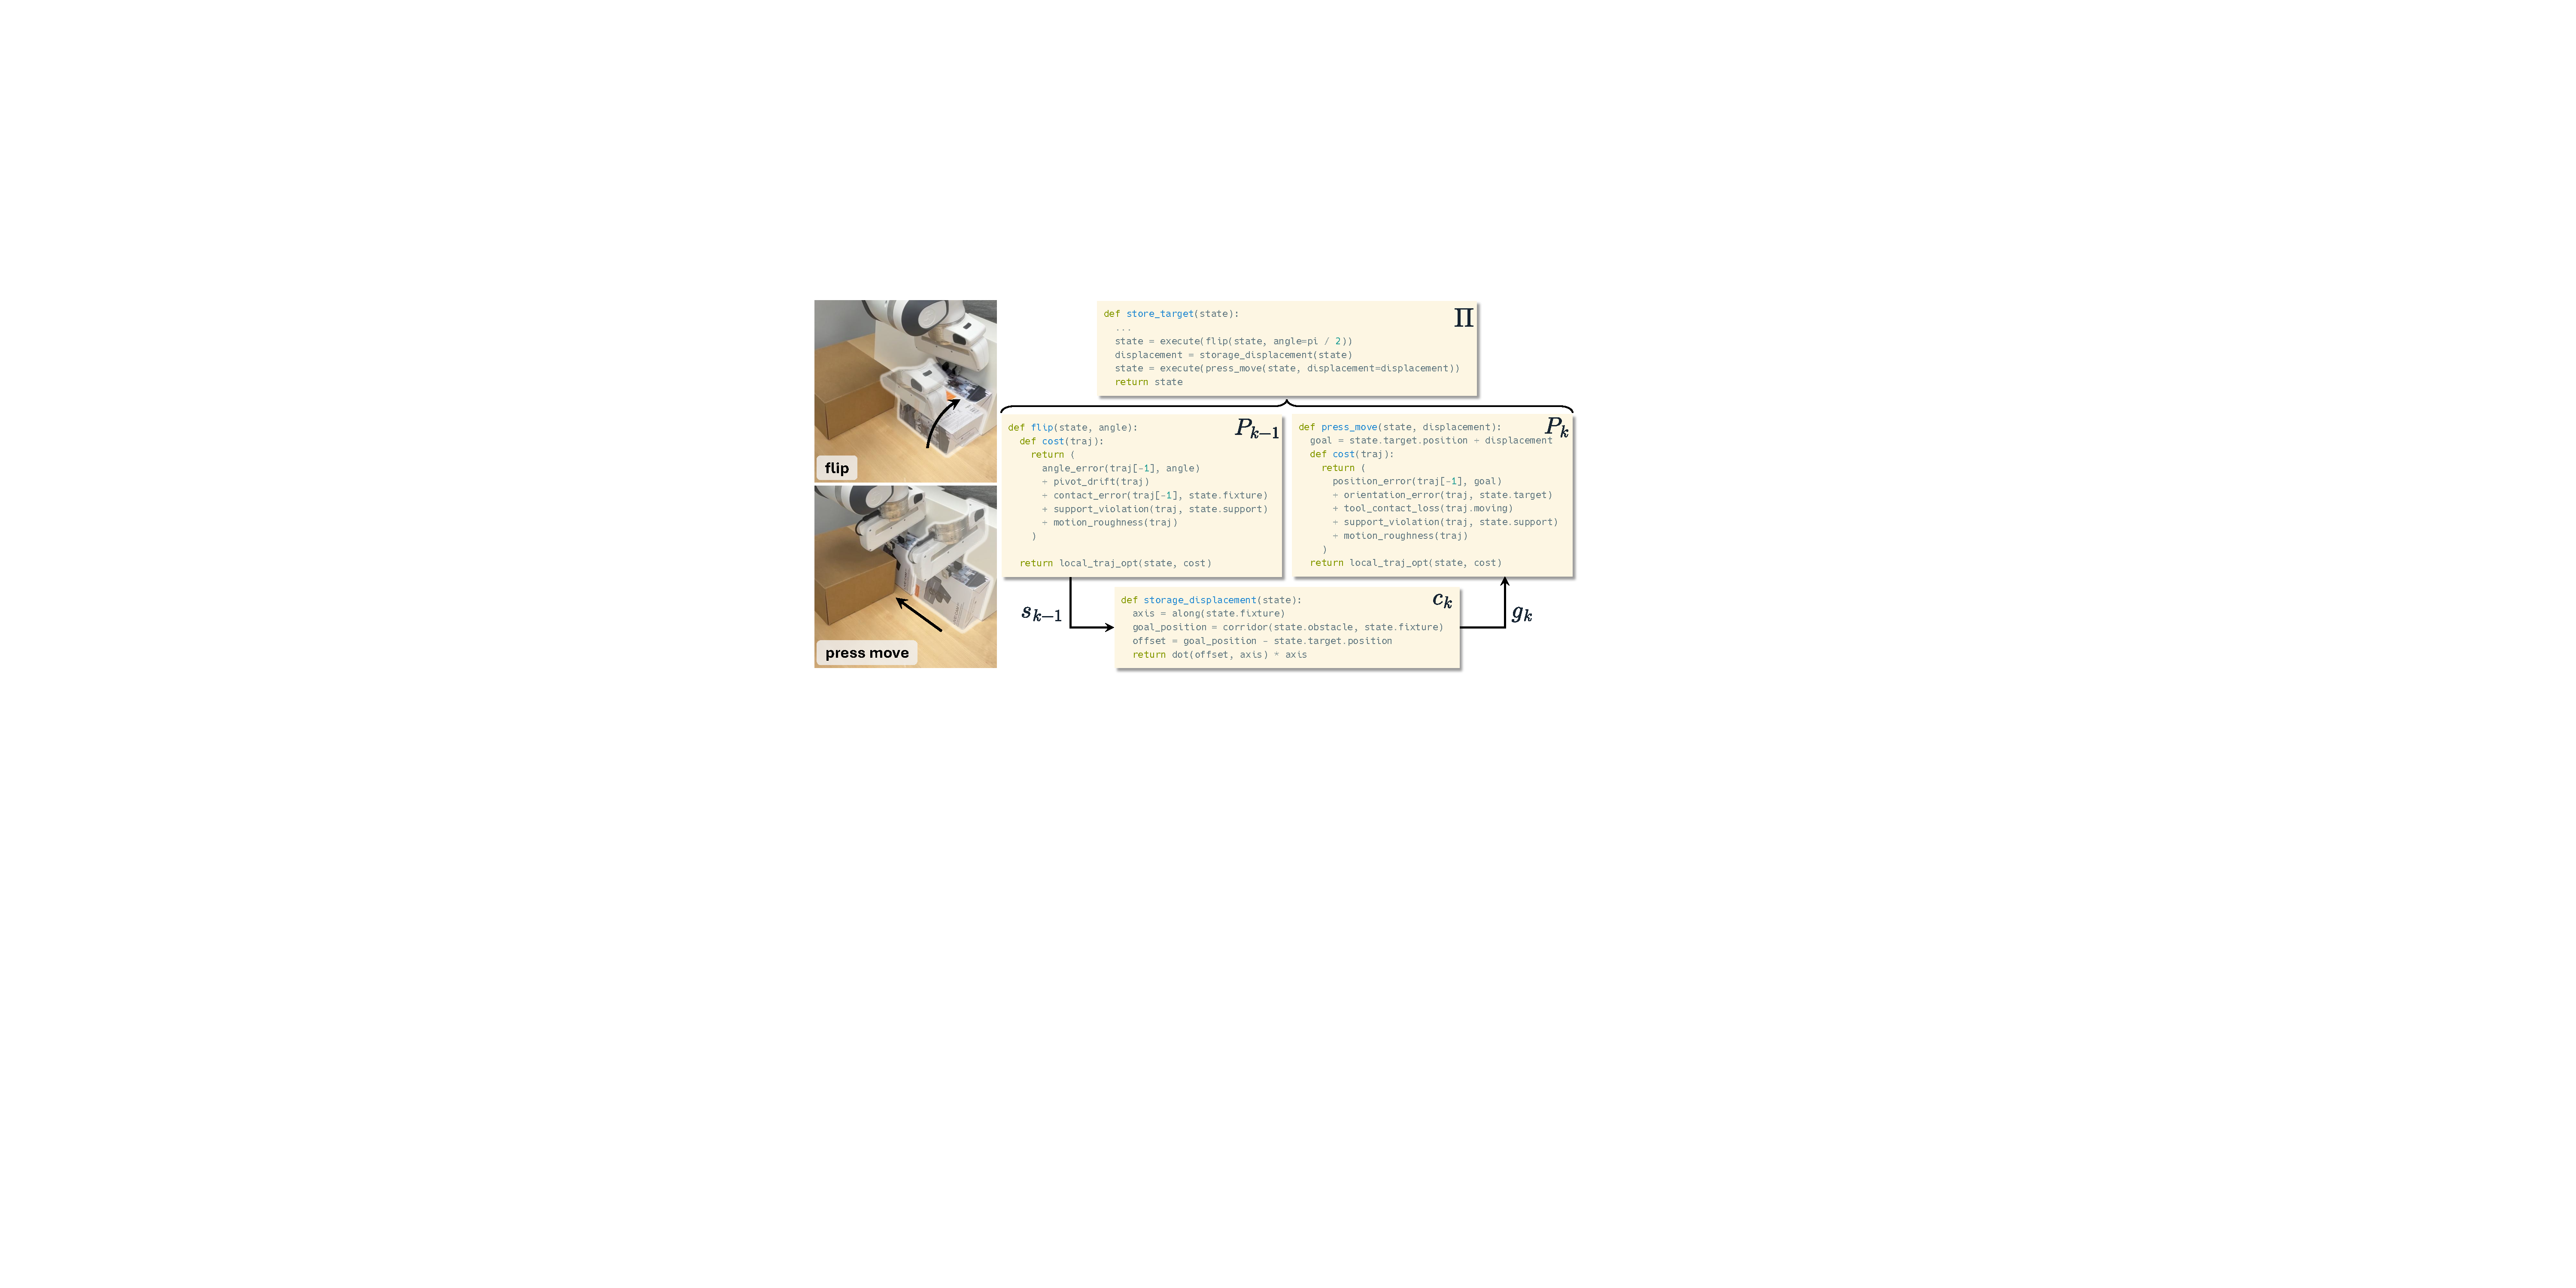
\includegraphics[width=\linewidth]{figures/program.pdf}
    \caption{\textbf{Composing primitives by relational constraints.}}
    \label{fig:program}
    \vspace{-0.3in}
\end{figure}

Suppose we have a library of primitives $\mathcal{P}$, where each $P_i \in \mathcal{P}$ realizes an object-level motion effect. A strategy $\Pi$ is a reusable task-level program that composes these primitives to accomplish an overall task. It specifies the sequence of primitives to invoke, how task roles map to each primitive, and how the requested effect of each invocation is determined:
\begin{equation*}
    \Pi
    = \left(G_\Pi,C_\Pi,\Psi_\Pi,
      \left\langle(P_{i_k},m_k,c_k)\right\rangle_{k=1}^{K}\right),
\end{equation*}
where $G_\Pi$ describes the overall task goal and $\Psi_\Pi$ evaluates its final outcome.

\xhdr{Strategy interface.}
A strategy exposes semantic roles and their required relations,
\begin{equation*}
    C_\Pi=(\mathbf{r}_\Pi,\Gamma_\Pi).
\end{equation*}
To invoke the strategy, a role binding $b\in\operatorname{Bind}_E(\mathbf{r}_\Pi,\Gamma_\Pi)$ assigns an entity to each strategy role while satisfying $\Gamma_\Pi$. Primitive effect parameters are not exposed through $C_\Pi$; instead, they are derived inside the strategy during execution.

\xhdr{Primitive Composition by Constraints.}
A strategy consists of $K$ phases, each represented by a tuple $(P_{i_k},m_k,c_k)$, where $P_{i_k} \in \mathcal{P}$ is a primitive, $m_k$ is a role map, and $c_k$ is a connecting constraint. For the invoked primitive $P_{i_k}$, $m_k$ produces a role binding $b_k$ that fills the role declarations $\mathbf{r}_{i_k}$, while $c_k$ produces an effect argument $g_k$ that fills the parameter declarations $\mathbf{q}_{i_k}$. The connecting constraint declaratively specifies how phase $k$ depends on the outcome of phase $k-1$ and is evaluated just in time at the beginning of phase $k$:
\begin{equation*}
    \begin{aligned}
        b_k&=m_k(b)
            \in\operatorname{Bind}_E(\mathbf{r}_{i_k},\Gamma_{i_k}),\\
        g_k&=c_k(E,s_{k-1},b)
            \in\operatorname{Val}(\mathbf{q}_{i_k}),
    \end{aligned}
\end{equation*}
where $s_{k-1}\in\mathcal{X}(E)$ denotes the environment state after the execution of phase $k-1$. The phase is then executed as
\begin{equation*}
    s_k=\operatorname{Exec}\!\left(
        P_{i_k};E,s_{k-1},g_k,b_k\right).
\end{equation*}
Here, $\operatorname{Exec}$ solves the local trajectory-optimization problem of $P_{i_k}$ and executes the optimized trajectory.

For example, Figure~\ref{fig:program} shows a \textit{press move} following a \textit{flip}. The role map $m_k$ maps the strategy's target object, supporting surface, and tool roles to the corresponding roles of the \textit{press-move} primitive, producing $b_k$. The connecting constraint $c_k$ determines the goal position from the relation between the brown obstacle and the white fixture. Using the target object's current position in the post-flip state $s_{k-1}$, it computes the displacement toward this goal along the fixture axis, producing the effect argument $g_k$ for the \textit{press move} primitive.

\subsection{Strategy Instantiation in Novel Scenes}
\label{sec:novel_instantiation}

To deploy a strategy in a novel scene, we only need to provide a semantic binding. Given a novel scene $E^\star$ and instruction $l^\star$, RAPID uses a coding agent to rapidly generate a semantic binding $b^\star \in\operatorname{Bind}_{E^\star}(\mathbf{r}_\Pi,\Gamma_\Pi)$ that assigns scene entities to the semantic roles exposed by the strategy interface.Since this step only associates the exposed semantic roles with scene entities, it is lightweight and incurs little deployment overhead. At phase $k$, the strategy derives the primitive binding and effect argument automatically. 

Throughout this process, the strategy program $\Pi$ and the referenced primitives remain frozen. Generalization therefore arises from the relational program representation, together with the adaptation of trajectory optimization to the geometry and physical properties of the new scene.

\section{Agentic Programming from Demonstration}
\label{sec:agentic_programming}

In Sec.~\ref{sec:relational_programs}, we introduced a reusable and generalizable representation of relational manipulation programs that can be efficiently instantiated in novel scenes. We now describe how RAPID employs a coding agent to construct and iteratively refine such programs from a single visual human demonstration. Specifically, RAPID closes the agentic loop with the single demonstration by automatically inferring the task specification, generating programs the manipulation primitives referred by the strategy, and reconstructing the interactive simulation environments used for verification.


\subsection{Reconstructing Interactive Environments}
\label{sec:loop_ingredients}

\xhdr{Interactive environment.}
To verify a manipulation program, RAPID reconstructs an interactive simulation environment from the initial RGB-D frame of the demonstration. We first use a vision-language model (VLM) to identify the objects in the scene, assign them with semantic labels, and estimate their physical properties. Then, for each semantic name, we utilize SAM~3~\cite{carion2026sam} to get a segmentation mask. The RGB-D frame and the mask are then fed into SAM~3D~\cite{chen2026sam} to reconstruct a complete mesh. Finally, we use FoundationPose~\cite{wen2024foundationpose} to register each mesh to the RGB-D frame, and assemble the reconstructed objects and robot model in MuJoCo~\cite{todorov2012mujoco}. The resulting environment preserves the scene entities, geometry, and spatial relations needed to execute the candidate program and evaluate its success predicates.

\xhdr{Feasible scene variants.}
Verifying a program only in the reconstructed environment from a single demonstration may leave accidental assumptions about the demonstration undetected. To improve reusablity and generalizability, RAPID uses a task-agnostic variation sampler to generate scene variants. This sampler will randomize object appearances, sizes, poses, as well as physical parameters such as mass, friction, and elasticity. However, the randomly sampled scenes might not be feasible for a certain primitive or strategy. Therefore, we will let the coding agent to write a filter to leave out those infeasible variants based on its understanding of the primitive or the strategy. A variant is accepted only if it preserves the declared roles and relations, retains the task meaning, and remains physically feasible. 

\subsection{Primitive Construction}
\label{sec:primitive_construction}
To construct the primitives, we first need to decompose the demonstration of the overall tasks into a sequence of interaction phases. Given the full demonstration $D$ and its natural language description $l$, RAPID calls a subagent to partition $D$ into an ordered sequence of interaction segments $(D_1,\ldots,D_K)$ and assigns a local description $l_i$ to each $D_i$. For each $(D_i,l_i)$, if the coding agent recognizes that the behavior is covered by an existing primitive in the primitive library $\mathcal{P}$, we can simply retrieve this primitive. Otherwise, the coding agent will infer a primitive specification consisting of a semantic goal $G_i$ and a success predicate $\Psi_i$ from $(D_i,l_i)$. It further reasons about the contact interactions that produces the demonstrated effect, the relational structure that should remain invariant across executions, and the quantities that might vary between invocations. For example, for the flipping primitive in Table~\ref{tab:flip_primitive}, the demonstrated rotation supplies the flipping-angle argument, while the required relations among the target, support, fixture, and pusher define the reusable interaction structure.

Given the inferred primitive specification and the analysis about physical interaction structure, the coding agent will generate the relational primitive contract $C_i$, geometry resolver $\rho_i$, and optimization cost $J_i$ introduced in Sec.~\ref{sec:relational_primitives}. RAPID then iteratively verifies and revises the resulting primitive in the reconstructed interactive environment $\widehat{E}_i$ as well as in automatically generated scene variants. The complete process is illustrated in Algorithm~\ref{alg:agentic_programming}: RAPID reconstructs the segment-level environment $\widehat{E}_i$, proposes a primitive program $P_i$, generates feasible scene variants, and revises the program until the success predicate $\Psi_i$ is satisfied across the verification set $\mathcal{V}_i$. Finally, the primitive is added to the library $\mathcal{P}$.

\subsection{Strategy Composition}
\label{sec:program_revision}

After constructing the required primitives, RAPID composes them into a task-level strategy. Given the full demonstration $D$ and instruction $l$, the coding agent infers a strategy specification consisting of the overall task goal $G_\Pi$ and final success predicate $\Psi_\Pi$. The sequence of the interaction segments $(D_1,\ldots,D_K)$ determines the ordering of the primitive composition. The agent then constructs the strategy interface $C_\Pi$ and, for each phase $k$, selects a verified primitive $P_{i_k}$, defines the role map $m_k$, and specifies the connecting constraint $c_k$. Together, these components form an initial version of the strategy $\Pi$. 

RAPID then iteratively verifies and revises the strategy in the reconstructed interactive environment $\widehat{E}_0$ and its feasible scene variants. As illustrated by Algorithm~\ref{alg:agentic_programming}, during each execution, RAPID binds the semantic roles, invokes the selected primitives sequentially, evaluates each connecting constraint just in time, and checks the final outcome with $\Psi_\Pi$. The failure signals are returned to the coding agent, and the coding agent will revise the strategy composition accordingly while keeping the verified primitives fixed, until $\Psi_\Pi$ is satisfied across $\mathcal{V}_\Pi$. 

\begin{algorithm}[t]
    \caption{RAPID}
    \label{alg:agentic_programming}
    \KwIn{Human demonstration $D$, instruction $l$}
    \KwOut{Verified primitives $\mathcal{P}$ and strategy $\Pi$}
    $\{(D_i,l_i)\}_{i=1}^{K}\gets\Call{Segment}{D,l}$\;
    $\mathcal{P}\gets\emptyset$\;
    \textcolor{black!70}{\textit{// Primitive construction}}\;
    \For{$i=1,\ldots,K$}{
        $\widehat{E}_i\gets\Call{Reconstruct}{D_i}$\;
        $(G_i,\Psi_i)\gets\Call{InferObjective}{D_i,l_i}$\;
        $g_i\gets\Call{InferEffect}{D_i,G_i}$\;
        $P_i\gets\Call{ProposePrimitive}{D_i,G_i,\Psi_i,\widehat{E}_i}$\;
        $\mathcal{V}_i\gets\{\widehat{E}_i\}\cup\Call{Variants}{\widehat{E}_i,P_i}$\;
        $P_i\gets\Call{VerifyRevise}{P_i,\mathcal{V}_i,(g_i,l_i)}$\;
        $\mathcal{P}\gets\mathcal{P}\cup\{\Call{Freeze}{P_i}\}$\;
    }
    \textcolor{black!70}{\textit{// Strategy composition}}\;
    $\widehat{E}_0\gets\Call{Reconstruct}{D}$\;
    $(G_\Pi,\Psi_\Pi)\gets\Call{InferObjective}{D,l}$\;
    $\Pi\gets\Call{Compose}{D,\mathcal{P},G_\Pi,\Psi_\Pi,\widehat{E}_0}$\;
    $\mathcal{V}_\Pi\gets\{\widehat{E}_0\}\cup\Call{Variants}{\widehat{E}_0,\Pi}$\;
    $\Pi\gets\Call{VerifyRevise}{\Pi,\mathcal{V}_\Pi,l}$\;
    \KwRet{$\mathcal{P},\Call{Freeze}{\Pi}$}\;
    \textcolor{black!70}{\textit{// Shared verification and revision}}\;
    \SetKwProg{Fn}{function}{}{}
    \Fn{\textnormal{\textsc{VerifyRevise}}$(Q,\mathcal{V},a)$}{
        \Repeat{$\Call{AllSuccessful}{\mathcal{R}}$}{
            $\mathcal{R}\gets\Call{ExecuteEvaluate}{Q,\mathcal{V},a}$\;
            \If{$\neg\Call{AllSuccessful}{\mathcal{R}}$}{
                $Q\gets\Call{DiagnoseRevise}{Q,\mathcal{R}}$\;
            }
        }
        \KwRet{$Q$}\;
    }
\end{algorithm}

\section{Experiments}

\begin{figure}[t]
    \centering
    \fbox{\parbox[c][2in][c]{0.96\linewidth}{
        \centering
        \textbf{Experiment Setting Placeholder}
    }}
    \caption{Experiment settings.}
    \label{fig:experiment_setting}
\end{figure}

\begin{table*}[t]
    \centering
    \caption{Experiment Results}
    \label{tab:experiment_results}
    % Previous layout (methods as rows and skeletons as columns):
% \resizebox{\textwidth}{!}{%
% \begin{tabular}{@{}l*{8}{c}@{}}
%     \toprule
%     \textbf{Task}
%         & \multicolumn{3}{c}{\textbf{Store Box}}
%         & \multicolumn{3}{c}{\textbf{Grasp Box}}
%         & \multicolumn{2}{c}{\textbf{Pick up Book}} \\
%     \cmidrule(lr){2-4}\cmidrule(lr){5-7}\cmidrule(l){8-9}
%     \textbf{Skeleton}
%         & push$\rightarrow$push
%         & press$\rightarrow$flip$\rightarrow$push
%         & rotate$\rightarrow$push$\rightarrow$push
%         & push$\rightarrow$flip$\rightarrow$grasp
%         & push$\rightarrow$flip$\rightarrow$press$\rightarrow$grasp
%         & press$\rightarrow$push$\rightarrow$flip$\rightarrow$grasp
%         & tilt$\rightarrow$grasp
%         & push$\rightarrow$grasp \\
%     \midrule
%     $\pi_{0.5}$                           & & & & & & & & \\
%     RAPID w/o primitive learning          & & & & & & & & \\
%     RAPID w/o optimization program        & & & & & & & & \\
%     RAPID w/o goal inferring              & & & & & & & & \\
%     RAPID w/o relational representation  & & & & & & & & \\
%     RAPID                                & & & & & & & & \\
%     \bottomrule
% \end{tabular}%
% }

{%
\small
\setlength{\tabcolsep}{6pt}
\renewcommand{\arraystretch}{1.08}
\begin{adjustbox}{max width=\linewidth}
\begin{tabular}{@{}ll*{6}{c}@{}}
    \toprule
    \textbf{Task}
        & \textbf{Skeleton}
        & $\pi_{0.5}$
        & \textbf{RAPID w/o Prim.}
        & \textbf{RAPID w/o Optim.}
        & \textbf{RAPID w/o Goal}
        & \textbf{RAPID w/o Rel.}
        & \textbf{RAPID} \\
    \midrule
    \multirow{3}{*}{Store Box}
        & push$\rightarrow$push & -- & -- & -- & -- & -- & -- \\
        & press$\rightarrow$flip$\rightarrow$push & -- & -- & -- & -- & -- & -- \\
        & rotate$\rightarrow$push$\rightarrow$push & -- & -- & -- & -- & -- & -- \\
    \midrule
    \multirow{3}{*}{Grasp Box}
        & push$\rightarrow$flip$\rightarrow$grasp & -- & -- & -- & -- & -- & -- \\
        & push$\rightarrow$flip$\rightarrow$press$\rightarrow$grasp & -- & -- & -- & -- & -- & -- \\
        & press$\rightarrow$push$\rightarrow$flip$\rightarrow$grasp & -- & -- & -- & -- & -- & -- \\
    \midrule
    \multirow{2}{*}{Pick up Book}
        & tilt$\rightarrow$grasp & -- & -- & -- & -- & -- & -- \\
        & push$\rightarrow$grasp & -- & -- & -- & -- & -- & -- \\
    \bottomrule
\end{tabular}
\end{adjustbox}
}

\end{table*}

\begin{table}[t]
    \centering
    \caption{Experiment Results on LIBERO-Pro}
    \label{tab:libero_pro_results}
    {%
\small
\setlength{\tabcolsep}{8pt}
\renewcommand{\arraystretch}{1.08}
\begin{adjustbox}{max width=\linewidth}
\begin{tabular}{@{}l*{6}{c}@{}}
    \toprule
    \multirow{2}{*}{\textbf{Method}}
        & \multicolumn{2}{c}{\textbf{libero-object}}
        & \multicolumn{2}{c}{\textbf{libero-goal}}
        & \multicolumn{2}{c}{\textbf{libero-spatial}} \\
    \cmidrule(lr){2-3}\cmidrule(lr){4-5}\cmidrule(l){6-7}
        & \textbf{Pos (Avg.)} & \textbf{Task (Avg.)}
        & \textbf{Pos (Avg.)} & \textbf{Task (Avg.)}
        & \textbf{Pos (Avg.)} & \textbf{Task (Avg.)} \\
    \midrule
    OpenVLA     & 0            & 0             & 0             & 0             & 0             & 0             \\
    $\pi_0$     & 0            & 0             & 0             & 0             & 0             & 0             \\
    $\pi_{0.5}$ & 0.17         & 0.01          & 0.38          & 0             & 0.20          & 0.01          \\
    CaP-Agent0  & 0.22         & 0.18          & 0.26          & 0.17          & 0.12          & 0.14          \\
    ASPIRE      & 0.98         & 0.95          & \textbf{0.81} & 0.45          & 0.51          & 0.60          \\
    RAPID       & \textbf{1}  & \textbf{0.95} & 0.67          & \textbf{0.53} & \textbf{0.83} & \textbf{0.81} \\
    \bottomrule
\end{tabular}
\end{adjustbox}
}

\end{table}

\begin{figure}[t]
    \centering
    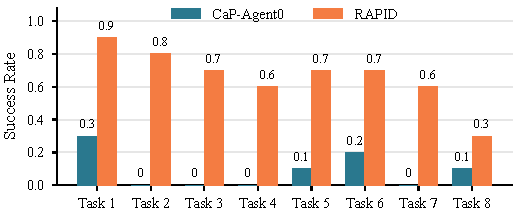
\includegraphics[width=\linewidth]{figures/real_world_results.pdf}
    \caption{Success rates across eight real-world manipulation tasks.}
    \label{fig:experiment_real}
\end{figure}

\section{Conclusion}
We presented \ours, a framework that closes the agentic coding loop for robotic manipulation from a single visual human demonstration and a language description. By automatically deriving task specifications, manipulation primitives, and interactive verification environments, \ours enables a coding agent to construct, execute, and iteratively refine reusable manipulation strategies. Our object-centric relational program representation represents manipulation primitives as trajectory-optimization programs and composes them with relational constraints, enabling generalization to novel scenes. Experiments on eight contact-rich nonprehensile manipulation tasks demonstrate strong generalization across object and scene variations, while evaluations on LIBERO-Pro and a real robotic system support \ours's broader applicability and practical deployment.

% \input{sections/8-Appendix}

\section*{ACKNOWLEDGMENT}
\xhdr{AI Disclosure.} The authors used OpenAI Codex~\cite{openai_codex} to assist with software implementation and debugging.

% Enable the bibliography after adding the first citation.
% \bibliographystyle{ieeetr}
\bibliographystyle{IEEEtran}
\bibliography{references,references_new}

\end{document}
